\documentclass[10pt]{article}
\usepackage[utf8x]{inputenc}
\usepackage{fullpage,fancyhdr}
\usepackage[pdftex]{graphicx}
\usepackage[usenames,dvipsnames]{color}
\usepackage{geometry}
\usepackage{graphicx,float,wrapfig}
\usepackage{amsmath,amsfonts,amsthm,amssymb}
\usepackage{listings}
\usepackage{courier}
\usepackage{ifthen}
\usepackage{setspace}
\usepackage{fancyhdr}
\usepackage{lastpage}
\usepackage{extramarks}
\usepackage{chngpage}
\usepackage{soul}
\DeclareGraphicsRule{.tif}{png}{.png}{`convert #1 `dirname #1`/`basename #1 .tif`.png}

\definecolor{lightgray}{gray}{0.5}
\definecolor{MyDarkGreen}{rgb}{0.0,0.4,0.0}

\topmargin=-0.45in      %
\evensidemargin=0in     %
\oddsidemargin=0in      %
\textwidth=6.5in        %
\textheight=9.0in       %
\headsep=0.25in         %
\headheight=12.0pt      %

% For faster processing, load Matlab syntax for listings
\lstloadlanguages{Matlab}%
\lstset{language=Matlab,
        frame=single,
        basicstyle=\ttfamily,
        keywordstyle=[1]\color{Blue}\bf,
        keywordstyle=[2]\color{Purple},
        keywordstyle=[3]\color{Blue}\underbar,
        identifierstyle=,
        commentstyle=\usefont{T1}{pcr}{m}{sl}\color{MyDarkGreen}\small,
        stringstyle=\color{Purple},
        showstringspaces=false,
        tabsize=5,
        % Put standard MATLAB functions not included in the default
        % language here
        morekeywords={xlim,ylim,var,alpha,factorial,poissrnd,normpdf,normcdf},
        % Put MATLAB function parameters here
        morekeywords=[2]{on, off, interp},
        % Put user defined functions here
        morekeywords=[3]{FindESS},
        morecomment=[l][\color{Blue}]{...},
        numbers=left,
        firstnumber=1,
        numberstyle=\tiny\color{Blue},
        stepnumber=5
        }

\pagestyle{fancyplain}
 
\fancyhf{}
 
\lhead{\fancyplain{}{Carroll, Jha}}
\chead{\fancyplain{}{ELEC6530 - Mobile Robot Design}}
\rhead{\fancyplain{}{\today}}
\rfoot{\fancyplain{}{\thepage\ of \pageref{LastPage}}}

%opening
\title{ELEC6530 Homework 2 - Differential Drive Kinematics}
\author{M. Carroll and N. Jha}
\date{}

\begin{document}

\maketitle

\section{Model Derivation}
\subsection{Kinematics - Body Frame}
First, we must derive the kinematics of the model in the body frame.  The coordinate frame of the robot is x forward, y left, and z up.  Theta represents the rotation of the body about the z-axis.  
The axes form a right-handed coordinate system, so positive theta indicates counter-clockwise rotation.

The velocity of the robot can be represented as a pair of vectors.  $\vec{v}$ represents the linear velocity (forwards and backwards) of the robot, and $\vec{w}$ represents the angular velocity (rotation)
of the robot.

Given $\omega_{R}$ and $\omega_{L}$, the wheel speeds of the right and left wheels, we can represent the linear and angular velocity of the differential drive robot as shown in Equation ~\ref{eqn:velocities}.

\begin{figure}[h]
 \centering
 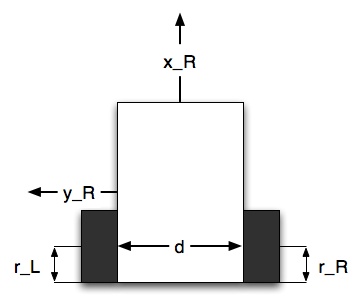
\includegraphics[scale=0.5,keepaspectratio=true]{./robot.png}
 % robot.png: 576x733 pixel, 72dpi, 20.32x25.86 cm, bb=0 0 576 733
 \caption{Physical Configuration of the Robot}
 \label{fig:robotparams}
\end{figure}

\begin{equation}
  \begin{aligned}
    v &= \dfrac{r_R}{2} \omega_R + \dfrac{r_L}{2} \omega_L \\
    w &= \dfrac{r_R}{d} \omega_R - \dfrac{r_L}{d} \omega_L
  \end{aligned}
  \label{eqn:velocities}
\end{equation}
\\
Where $r_{R}$ and $r_{L}$ are the wheel radii of the left and right wheels, and $d$ is the width of the wheelbase as shown in Figure ~\ref{fig:robotparams}.

\newpage
\subsection{Kinematics - Inertial Frame}
The next step is to derive the kinematics of the robot in the global coordinate frame.  The global coordinate frame is represented in Figure ~\ref{fig:global}.

\begin{figure}[h]
 \centering
 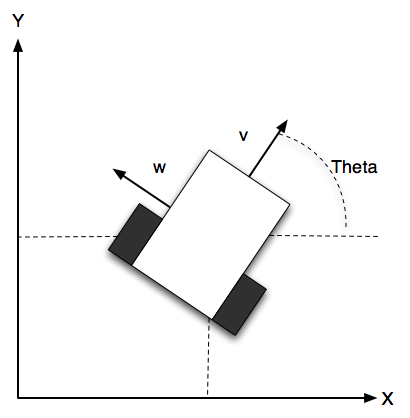
\includegraphics[scale=0.4,keepaspectratio=true]{./global.png}
 % global.png: 410x418 pixel, 72dpi, 14.46x14.74 cm, bb=0 0 410 418
 \caption{Robot in the Inertial Coordinate Frame}
 \label{fig:global}
\end{figure}

Since v and w are velocities, it is possible to derive the velocity and angular velocity of the robot in the inertial coordinate frame.  The equations of motion are derived in Equation ~\ref{eqn:global}.

\begin{equation}
\begin{align}
\dot{x} &= v \cos{\theta} \\
\dot{y} &= v \sin{\theta} \\
\dot{\theta} &= \omega
\end{align}
\label{eqn:global}
\end{equation}

To find the position of the robot, then these time-differentials must be integrated from a beginning time $T_{0}$ to the current time $T$.  Additionally, a constant offset may be added if the robot does not start
at the origin of the intertial coordinate frame. These integrals are performed in Equation~\ref{eqn:integration}.

\begin{equation}
\begin{align}
 x(t) &= \int_{T_{0}}^{T} v(t) \cos{(\theta(t))} dt + X_{0} \\
 y(t) &= \int_{T_{0}}^{T} v(t) \sin{(\theta(t))} dt + Y_{0} \\
 \theta(t) &= \int_{T_{0}}^{T} w(t) dt + \theta_{0}
\end{align}
\label{eqn:integration}
\end{equation}

\subsection{Discrete Time Model}
Often, it is more useful to represent the kinematics of the robot via a discrete-time model.  This model assumes that the continuous values of the motor speeds are sampled at a 
constant rate $1/\Delta t$ and represented as $v_k$ and $w_k$.  This makes the equations of motion as in Equation~\ref{eqn:discrete}.

\begin{equation}
 \begin{bmatrix}
  x \\ y \\ \theta
 \end{bmatrix}_{k+1} = 
 \begin{bmatrix}
  x \\ y \\ \theta
 \end{bmatrix}_{k} + 
 \begin{bmatrix}
  \Delta t v_k \cos{(\theta_k + \Delta t w_k/2)}\\
  \Delta t v_k \sin{(\theta_k + \Delta t w_k/2)}\\
  \Delta t w_k
 \end{bmatrix}
\label{eqn:discrete}
\end{equation}

\clearpage
\section{Simple Tests of Kinematic Model}
\subsection{Equal, Contant Wheel Velocities}
Basic intuition tells us that if both wheels are at the same speed, then the robot will drive in a straight line in the direction that it started in.  This can be seen from our simulation results below.

The robot was started heading towards 0 degrees (the x-axis), and then each wheel was commanded to the same speed.  The robot travels in the x-direction throughout the entire simulation.

Figure~\ref{fig:equalconstantpose} shows the x,y, and theta values of the pose of the robot over time, while Figure~\ref{fig:equalconstantplane} shows the top-down view of the robot's motion.

\begin{figure}[h]
 \centering
 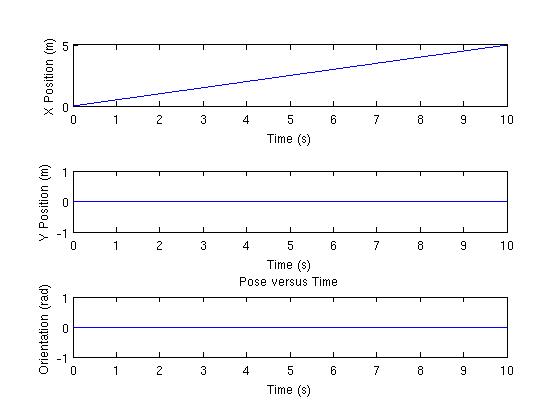
\includegraphics[scale=0.55,keepaspectratio=true]{equalconstantpose.png}
 \caption{Pose of the Robot vs Time with Equal, Constant Wheel Speeds}
 \label{fig:equalconstantpose}
\end{figure}

\begin{figure}[h]
 \centering
 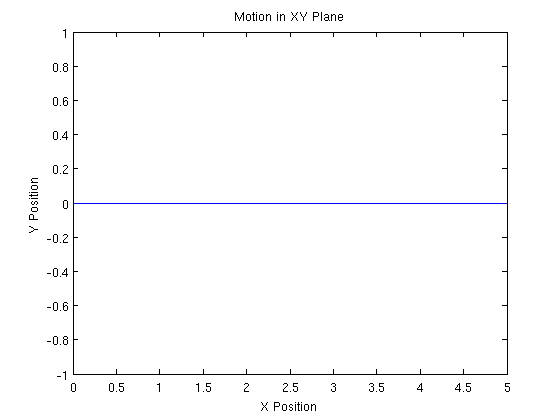
\includegraphics[scale=0.55,keepaspectratio=true]{equalconstantplane.png}
 \caption{Top-Down view of Robot Motion with Equal, Constant Wheel Speeds}
 \label{fig:equalconstantplane}
\end{figure}


\newpage
\subsection{Unequal, Constant Wheel Velocities}
Once again, intuition tells us that if one wheel rotates faster than the other, the robot will drive in a large arc, and given enough time, a circle.  This can bee seen from our simulation results below.

The robot was started heading towards 0 degrees (the x-axis), and the right wheel was commanded to faster than the left wheel by a factor of 5.  The robot travels in a circle.

Figure~\ref{fig:unequalconstantpose} shows the x,y, and theta values of the pose of the robot over time, while Figure~\ref{fig:unequalconstantplane} shows the top-down view of the robot's motion.

\begin{figure}[h]
 \centering
 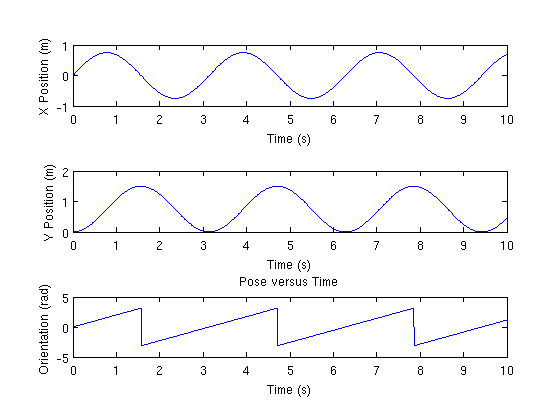
\includegraphics[scale=0.55,keepaspectratio=true]{unequalconstantpose.png}
 \caption{Pose of the Robot vs Time with Unequal, Constant Wheel Speeds}
 \label{fig:unequalconstantpose}
\end{figure}

\begin{figure}[h]
 \centering
 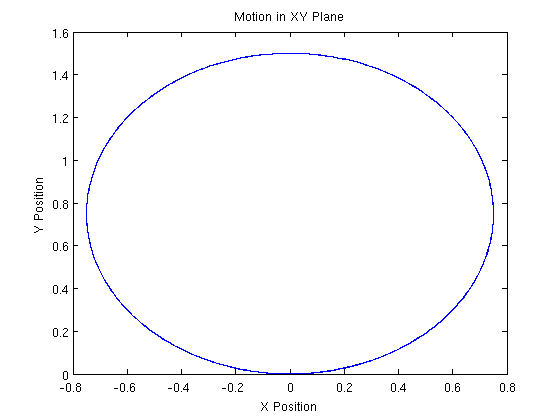
\includegraphics[scale=0.55,keepaspectratio=true]{unequalconstantplane.png}
 \caption{Top-Down view of Robot Motion with Unequal, Constant Wheel Speeds}
 \label{fig:unequalconstantplane}
\end{figure}

\newpage
\subsection{Equal, Noisy Wheel Velocities}
For a better test of the simulation, we also added in unit normally-distributed noise to the motor velocity commands to see the effect.

When the wheels were commanded to an equal velocity before the noise was applied, the robot ``wandered'' to the left and right of the x-axis line, but generally stayed around it.

Figure~\ref{fig:equalnoisepose} shows the x,y, and theta values of the pose of the robot over time, while Figure~\ref{fig:equalnoiseplane} shows the top-down view of the robot's motion.

\begin{figure}[h]
 \centering
 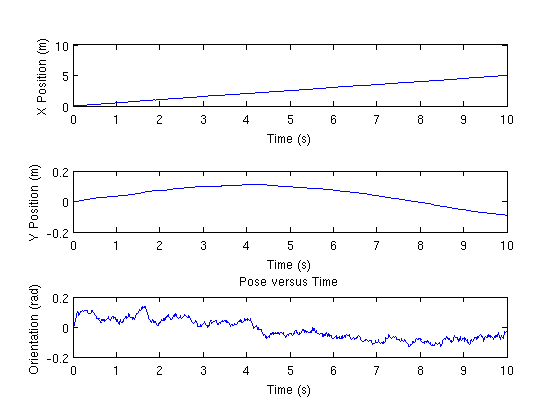
\includegraphics[scale=0.55,keepaspectratio=true]{equalnoisepose.png}
 \caption{Pose of the Robot vs Time with Equal, Noisy Wheel Speeds}
 \label{fig:equalnoisepose}
\end{figure}

\begin{figure}[h]
 \centering
 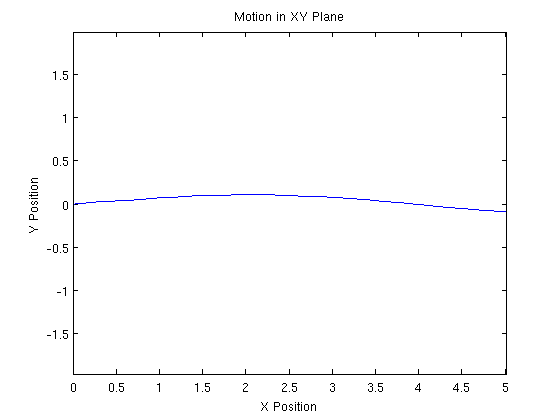
\includegraphics[scale=0.55,keepaspectratio=true]{equalnoiseplane.png}
 \caption{Top-Down view of Robot Motion with Equal, Noisy Wheel Speeds}
 \label{fig:equalnoiseplane}
\end{figure}


\newpage
\subsection{Unequal, Noisy Wheel Velocities}
When the wheels were commanded to an unequal velocity before the noise was applied, the robot ``wandered'' around a circular path, but couldn't repeat the path in multiple rotations.

Figure~\ref{fig:unequalnoisepose} shows the x,y, and theta values of the pose of the robot over time, while Figure~\ref{fig:unequalnoiseplane} shows the top-down view of the robot's motion.

\begin{figure}[h]
 \centering
 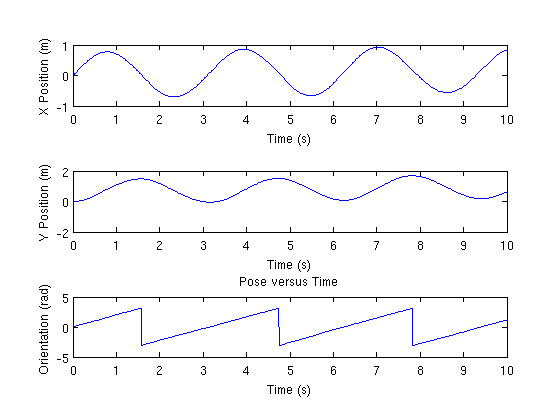
\includegraphics[scale=0.55,keepaspectratio=true]{unequalnoisepose.png}
 \caption{Pose of the Robot vs Time with Unequal, Noisy Wheel Speeds}
 \label{fig:unequalnoisepose}
\end{figure}

\begin{figure}[h]
 \centering
 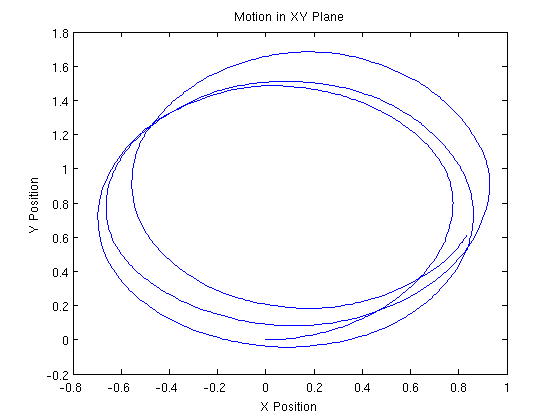
\includegraphics[scale=0.55,keepaspectratio=true]{unequalnoiseplane.png}
 \caption{Top-Down view of Robot Motion with Unequal, Noisy Wheel Speeds}
 \label{fig:unequalnoiseplane}
\end{figure}

\newpage
\section{MATLAB Simulation Code}

\lstinputlisting[language=Matlab]{../simulator.m}

\end{document}
